\documentclass[handout]{beamer}
\usepackage[utf8]{inputenc}
\usepackage[T2A]{fontenc}
\usepackage[english]{babel}
\usepackage{graphicx}
\usepackage{array}
\usetheme{Warsaw}
\usecolortheme{wolverine}

\usepackage{listings}
\usepackage{color}
\usepackage{amsmath}
\usepackage{changepage}

\definecolor{dkgreen}{rgb}{0,0.6,0}
\definecolor{gray}{rgb}{0.5,0.5,0.5}
\definecolor{mauve}{rgb}{0.58,0,0.82}

\lstset{
  language=Haskell,
  showstringspaces=false,
  columns=flexible,
  basicstyle={\small\ttfamily},
  numbers=none,
  numberstyle=\tiny\color{gray},
  keywordstyle=\color{blue},
  commentstyle=\color{dkgreen},
  stringstyle=\color{mauve},
  breaklines=true,
  breakatwhitespace=true,
  tabsize=2
}

\title{Optimizing compiler}
\author[Andrew Lelechenko]{Andrew Lelechenko \\ \texttt{1@dxdy.ru}}
\date{\#kievfprog, Kiev, 18.03.2017}

\begin{document}

\begin{frame}
	\titlepage
\end{frame}

\begin{frame}

\begin{figure}[H]
\centering
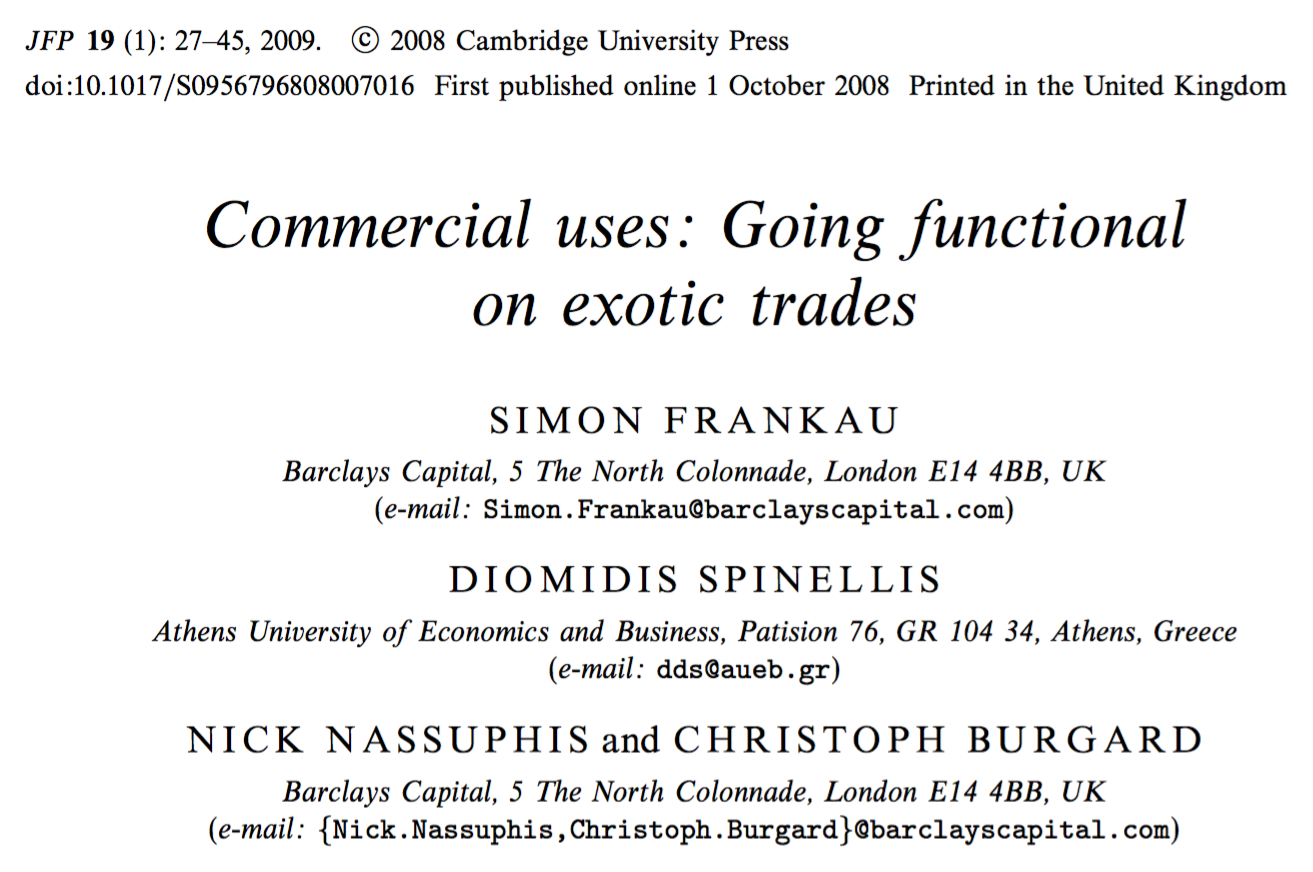
\includegraphics[width=\textwidth]{paper.png}
\end{figure}
\end{frame}

\begin{frame}{Papers and slides}

\begin{itemize}
\item Simon Frankau, Diomidis Spinellis, Nick Nassuphis, Christoph Burgard.
      {\em Commercial Uses: Going Functional on Exotic Trades.}
      J. Funct. Program. 19, 1, 27--45.

\bigskip

\item Tim Williams. {\em Exotic Tools for Exotic Trades} @ CodeMesh 2013.

\item Tim Williams, Peter Marks. {\em Structural Typing for Structured Products}
      @ Haskell Exchange 2014.
\end{itemize}

\end{frame}

\begin{frame}{Why not Haskell?}

\begin{itemize}

\item Haskell is an amazing language for writing your own compiler.

\item A rich ecosystem of libraries dedicated to compiler-related tasks.

\item A really powerful type system that can eliminate large classes of errors at compile time.

\item Many excellent educational resources for compiler writers:
      \begin{itemize}
      \item Stephen Diehl. {\em Write You a Haskell.}
      \item Andres Löh, Conor McBride, Wouter Swierstra. {\em A Tutorial Implementation of a Dependently Typed Lambda Calculus.}
      \end{itemize}

\item Compilers, written in Haskell: GHC, Elm, Purescript, Idris, Agda...
\end{itemize}

\end{frame}

\begin{frame}{SIMPL --- Simple IMPerative Language}

\begin{itemize}

\item Scalar and vector {\tt Double}-valued variables: {\tt a}, {\tt b[i]}, {\tt c[i][j]}.

\item Vector length is statically known beforehand.

\item Arithmetic operators, comparisons and ternary operator.

\item Only {\tt for}-loops without preliminary {\tt break}.

\item Basically, its computational power is equivalent to Excel sheet.

\item Powerful enough for physical/financial Monte-Carlo simulations with calculations repeated over random inputs and step-by-step time.

\end{itemize}

\centerline{Why not Fortran?}

\end{frame}

\begin{frame}[fragile]{Example: $n$-body problem, {\normalsize youtube.com/embed/qIVe\_xEv6zQ}}

\begin{itemize}
\item {\tt m[i]} is the mass of {\tt i}-th object (is known in compile time),
\item {\tt x[i]} and {\tt y[i]} are its coordinates,
\item {\tt vx[i]} and {\tt vy[i]} are its velocities by X- and Y-axis,
\item {\tt ax[i]} and {\tt ay[i]} are its accelerations.
\end{itemize}

\begin{lstlisting}
dt = 0.001
G  = 6.67e-11
foreach i in 1..n
  ax[i] = 0
  ay[i] = 0
  foreach j in 1..n
    d[i][j] = (x[i] - x[j]) ^ 2 + (y[i] - y[j]) ^ 2
    ax[i] = ax[i] - G * m[j] * (x[i]-x[j]) / d[i][j] ^ 3/2
    ay[i] = ay[i] - G * m[j] * (y[i]-y[j]) / d[i][j] ^ 3/2
foreach i in 1..n
  vx[i] = vx[i] + ax[i] * dt
  vy[i] = vy[i] + ay[i] * dt
   x[i] =   x[i] + vx[i] * dt
   y[i] =   y[i] + vy[i] * dt
\end{lstlisting}

\end{frame}

\begin{frame}[fragile]{Abstract syntax tree: types}

\vspace{-1ex}

Loop counters and variables are annotated with sizes on type level.

\begin{lstlisting}
data Counter (range :: Nat) = Counter String
data Reference (arity :: [Nat]) where
  V    :: String -> Reference xs
  (:!) :: Reference (x : xs) -> Counter x -> Reference xs
\end{lstlisting}

Expressions are simple:

\begin{lstlisting}
data Expr a where
  Ref  :: Reference '[] -> Expr Double
  Num  :: Double -> Expr Double
  (:+) :: Expr Double -> Expr Double -> Expr Double
  (:*) :: Expr Double -> Expr Double -> Expr Double
  (:^) :: Expr Double -> Expr Double -> Expr Double
  (:<) :: Expr Double -> Expr Double -> Expr Bool
  If   :: Expr Bool -> Expr a -> Expr a -> Expr a
\end{lstlisting}

And statements are even simpler:

\begin{lstlisting}
data Stmt where
  (:=) :: Reference '[] -> Expr Double -> Stmt
  For  :: Counter x -> [Stmt] -> Stmt
\end{lstlisting}

\end{frame}

\begin{frame}[fragile]{Abstract syntax tree: utils}

\begin{lstlisting}
instance Num (Expr Double) where
  (+) = (:+)
  (*) = (:*)
  negate x = x :* (-1)
  abs x    = If (x :< 0) (negate x) x
  signum x = If (x :< 0) (-1) (If (0 :< x) 1 0)
  fromInteger = Num . fromInteger
\end{lstlisting}

\begin{lstlisting}
(&&) :: Expr Bool -> Expr Bool -> Expr Bool
a && b = If a b a
\end{lstlisting}

\begin{lstlisting}
(||) :: Expr Bool -> Expr Bool -> Expr Bool
a || b = If a a b
\end{lstlisting}

\end{frame}

\begin{frame}[fragile]{Code example}

For a given {\tt c} build a vector {\tt [c, c+1...]}, square up its elements and return their sum.

\begin{lstlisting}
[ For i
  [ a!i := Ref c
  , c   := Ref c + 1 ]
, For i
  [ b!i := Ref (a!i) :^ 2 ]
, ret   := 0
, For i
  [ ret := Ref ret + Ref (b!i) ] ]
where a = "a"; b = "b"; c = "c"; ret = "ret"; i = "i"
\end{lstlisting}

Optimized:

\begin{lstlisting}
[ ret   := 0
  For i
  [ ret := Ref ret + Ref c :^ 2
  , c   := Ref c + 1 ]
where c = "c"; ret = "ret"; i = "i"
\end{lstlisting}

\end{frame}

\begin{frame}{Compiler's architecture}

\begin{tabular}{l@{~~~$\to$~~~}c@{~~~$\to$~~~}r}
Lexer/Parser &
Abstract Syntax Tree &
Code Generator \\ \hline
{\tt parsec}, &
optimizations &
ASM, C--, LLVM, \\
{\tt alex} / {\tt happy} &
&
C, JavaScript
\end{tabular}

\begin{figure}[H]
\centering
\colorbox{black}{
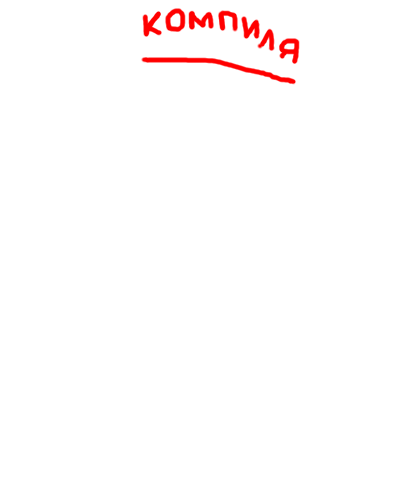
\includegraphics[width=0.4\textwidth]{plan.png}
}
\end{figure}

\end{frame}

\begin{frame}{Marginalia: lexer and parser}

Semantically:
\begin{itemize}
\item Lexer reads a list of tokens.
\item Parser transforms tokens into syntax tree.
\end{itemize}

Grammars:
\begin{itemize}
\item Lexer reads a regular grammar (regexp without backtracking).
\item Parser reads a context-free grammar (can parse nested brackets).
\item parsec can read even a context-sensitive grammar.
\end{itemize}

Static advantages:
\begin{itemize}
\item Lexer generates a very efficient finite automaton.
\item Parser checks grammar for ambiguities.
\end{itemize}

\end{frame}

\begin{frame}{Gentle optimizations}

We are interested in optimizations of SIMPL such that
\begin{itemize}
\item no auxiliary statements or variables are introduced,
\item expressions are replaced with equivalent in runtime ones.
\end{itemize}

We cannot:
\begin{itemize}
\item dismantle expressions into three-address code: \par
      {\tt x = y * 3 + 2} $\not\Longrightarrow$ {\tt t = y * 3; x = t + 2}.
\item dismantle loops into blocks, labels and gotos;
\item use Single Static Assignment or Continuation Passing Style.
\end{itemize}

We are free to
\begin{itemize}
\item rewrite expressions;
\item eliminate dead statements;
\item shuffle statements both top-down and inside-out;
\item detect high-level patterns such as maps and folds.
\end{itemize}

\end{frame}

\begin{frame}{Local optimizations}

Despite SIMPL is an imperative language with global side effects,
its expressions are pure and has no effects.

\begin{itemize}
\item Constant folding: \par
      {\tt 2 :* 3} $\Longrightarrow$ {\tt 6}.

\item Short circuiting: \par
      {\tt If (0 :< 1) a b} $\Longrightarrow$ {\tt b}.

\item Algebraic simplifications: \par
  {\tt x :+ 0} $\Longrightarrow$ {\tt x}, {\tt x :* 0} $\Longrightarrow$ {\tt 0}.

\item Reassociation and redistribution: \par
  {\tt (x :+ 2) :+ 3} $\Longrightarrow$ {\tt x :+ (2 :+ 3)} $\Longrightarrow$ {\tt x :+ 5}, \par
  {\tt (x :+ 3) :* 2} $\Longrightarrow$ {\tt x :* 2 :+ 3 :* 2} $\Longrightarrow$ {\tt x :* 2 :+ 6}.

\end{itemize}

\end{frame}

\begin{frame}[fragile]{Dead code: a time to keep, and a time to cast away}

\begin{itemize}

\item Detect statements, which can be entirely removed.

\item The analysis goes {\em backwards} in terms of control flow, from the return statement up to the start.

\item Transform as you go: if left-hand side reference is not {\em live set}, remove the statement at once. Otherwise remove LHS reference from {\em live set} and add RHS references.

\end{itemize}

\begin{lstlisting}
           -- Live set
a = 1      -- {}
b = a + 2  -- {a}, remove
c = a + 3  -- {a}
d = b * 2  -- {c}, remove
ret = c    -- {c}
           -- {ret}
\end{lstlisting}

\end{frame}

\begin{frame}[fragile]{Dead code: loops}
\begin{adjustwidth}{-1em}{-1em}

\begin{itemize}
\item Loops change control flow and are executed one or more times.
\item Perform a dummy backward pass without striping of statements to collect circular references.
\item Then unite obtained live set with the live set at the end of loop and perform actual pass.
\end{itemize}

\bigskip

\begin{tabular}{l@{}r}

\begin{lstlisting}
a = 0           -- {}
for i
  b[i] = a      -- {a} / {a}
  a = b[i] + 1  -- {b} / {b}
end             -- {b} / {a, b}
r = 0           -- {b}
for i
  r = r + b[i]  -- {r, b} / {r, b}
end             -- {r}    / {r, b}
\end{lstlisting}

&

\begin{lstlisting}
a = 0           -- {}, remove
for i
  b[i] = a      -- {} / {}, remove
  a = b[i] + 1  -- {} / {}, remove
end             -- {} / {}
r = 0           -- {}
                -- {r}
\end{lstlisting}

\end{tabular}

\end{adjustwidth}
\end{frame}

\begin{frame}[fragile]{Inlining: a time to rend, and a time to sew}

\begin{itemize}
\item Substitute RHS expression instead of LHS reference.
\item The analysis goes {\em forward} in terms of control flow.
\item Transform as you go: use the result of inlining for further substitutions.
\end{itemize}

Use cases:

\begin{itemize}
\item Always inline, when RHS is a constant or a reference.
\item Always inline live variables, which are consumed only once.
      \begin{lstlisting}
      data Liveness = One | Many
      instance Semigroup Liveness where
        _ <> _ = Many
      \end{lstlisting}
\item Inline if it gives way to non-growing expression after local optimizations.
\end{itemize}

\end{frame}

\begin{frame}[fragile]{Inlining: example}
\begin{adjustwidth}{-1.5em}{-1.5em}

\begin{lstlisting}
a = 2                  a = 2
b = x + a              b = x + 2 -- inline constants
c = b                  c = x + 2 -- b is a one-shot variable
d = c + 1              d = x + 3 -- non-growing local optimizations
e = c * 2              e = c * 2 --  x * 2 + 4 is larger
f = c ^ 3              f = c ^ 3 -- (x + 2) ^ 3 is larger
g = d * e * f * f      g = (x + 3) * (c * 2) * f * f
                                  -- d and e are one-shot variables
\end{lstlisting}

\end{adjustwidth}
\end{frame}

\begin{frame}[fragile]{Loop fusion: a time to break down and a time to build up}

\begin{itemize}

\item Detect maps and folds in imperative code. Loops, which effect is invariant to permutation of iterations' order, are {\tt map}. Other loops are {\tt fold}.

\item Fuse using {\tt map/map} and {\tt map/fold} rules.
\end{itemize}

\begin{lstlisting}
for i
  y[i] = x[i] * 2
for i
  z[i] = y[i] * 3
\end{lstlisting}

\centerline{map f . map g = map (f . g)}

\begin{lstlisting}
for i
  y[i] = x[i] * 2
  z[i] = y[i] * 3
\end{lstlisting}

\end{frame}

\begin{frame}[fragile]{Loop fusion: {\tt map/fold} rule}

\begin{lstlisting}
for i
  y[i] = x[i] * 2
ret = 0
for i
  ret = ret + y[i] * 3
\end{lstlisting}

Shuffle blocks:

\begin{lstlisting}
ret = 0
for i
  y[i] = x[i] * 2
for i
  ret = ret + y[i] * 3
\end{lstlisting}

\centerline{foldr f x . map g = foldr (f . g) x}

\begin{lstlisting}
ret = 0
for i
  y[i] = x[i] * 2
  ret = ret + y[i] * 3
\end{lstlisting}

\end{frame}

\begin{frame}[fragile]{Loop fission - 1}

\begin{lstlisting}
ret = 0
for i
  y[i] = x[i] * 2
  ret = ret * 2 + y[i]
for i
  z[i] = y[i] * 3
\end{lstlisting}

Distribute first loop:

\begin{lstlisting}
ret = 0
for i y[i] = x[i] * 2
for i ret = ret * 2 + y[i]
for i z[i] = y[i] * 3
\end{lstlisting}

Shuffle blocks:

\begin{lstlisting}
ret = 0
for i y[i] = x[i] * 2
for i z[i] = y[i] * 3
for i ret = ret * 2 + y[i]
\end{lstlisting}

\end{frame}

\begin{frame}[fragile]{Loop fission - 2}

\begin{lstlisting}
ret = 0
for i y[i] = x[i] * 2
for i z[i] = y[i] * 3
for i ret = ret * 2 + y[i]
\end{lstlisting}

Apply {\tt map/map} rule:

\begin{lstlisting}
ret = 0
for i
  y[i] = x[i] * 2
  z[i] = y[i] * 3
for i
  ret = ret * 2 + y[i]
\end{lstlisting}

Apply {\tt map/fold} rule:

\begin{lstlisting}
ret = 0
for i
  y[i] = x[i] * 2
  z[i] = y[i] * 3
  ret = ret * 2 + y[i]
\end{lstlisting}

\end{frame}

\begin{frame}
\centerline{\Huge\bf Thank you!}
\end{frame}

\end{document}
